\chapter{Experiments}
\label{ch:Experiments}

% TODO: refine this section to also be able to include experiments on MuST-SHE and other 
% - Base Experiment (challenge set)
% - Real-world Experiment (natural corpora)
% (-) WSD Experiment

We follow three main steps in doing the experiments. First, we preprocess the data, then we translate it, and lastly we evaluate the translations based on different factors.

%%%%%%%%%%%%%%%%%%%%%%%%%%%%%%%%%%%%%%%%%%%%%%%%%%%%%%%%%%%%%%%%%%%%%%%%%%%%%%%%%%%%%%%%%%%%
\section{Data Pre-processing}

As we can see in Subsection \ref{sec:Experiments:Challenge_Set}, the sentences in WinoMT usually consist of two gender ambiguous occupations and a context, containing disambiguation information about one of the occupations. We take the following steps to preprocess the sentences:

\begin{enumerate}
  \item \textbf{Sentence Extraction:}  
  In order to obtain fully ambiguous sentences, we remove the context information from the sentences and obtain a subset of 335 sentences from the type: "The developer argued with the designer.".
  To remove additional detection overhead, we want to have a single ambiguous word per sentence. For this purpose, we replace the second ambiguous word with a non-ambiguous proper noun, e.g. "John". 
  \item \textbf{Disambiguation:} 
  As next, we generate a new set of sentences, replacing the ambiguous word with a disambiguated version. We disambiguate the ambiguous word with different techniques:
  \begin{itemize}
      \item \textbf{Gender Forcing:} We use the gender-defining adjectives \textit{male} and \textit{female} in front of the gender-ambiguous word. This technique is meant to force the translator to make the right decision regarding gender.
      \item \textbf{Common Words Disambiguating:} We replace the ambiguous word with the following common gender non-ambiguous words: \textit{man, woman, girl, guy, boy}. This method serves as a baseline for comparison against the disambiguated occupations.
  \end{itemize}
\end{enumerate}

Table \ref{tab:preprocessing} shows the generated subsets obtained by disambiguating the base ambiguous sentence "The developer argued with John.".

\begin{table}
    \label{tab:preprocessing}
    \begin{tabularx}{\linewidth}{|l|X|l|}
        \hline
        \textbf{Disambiguation Method} & \textbf{Source Sentence} & \textbf{Source Word} \\ \hline
        Gender Forcing & The \textbf{male developer} argued with John. & developer \\
        & The \textbf{female developer} argued with John. & developer \\ \hline
        Common Words & The \textbf{man} argued with John. & man \\
        & The \textbf{woman} argued with John. & woman \\
        & The \textbf{girl} argued with John. & girl \\
        & The \textbf{guy} argued with John. & guy \\
        & The \textbf{boy} argued with John. & boy \\ \hline
    \end{tabularx}
    \caption{Example: Disambiguation subsets for the baseline sentence "The developer argued with John."}
\end{table}

%%%%%%%%%%%%%%%%%%%%%%%%%%%%%%%%%%%%%%%%%%%%%%%%%%%%%%%%%%%%%%%%%%%%%%%%%%%%%%%%%%%%%%%%%%%%
\section{Translation}

The next step in conducting the experiments is translating the subsets of sentences. This is executed in two steps:

\begin{enumerate}
    \item \textbf{Translation Source -> Target:} 
    First, the subsets are translated in the target language.
    \item \textbf{Backtranslation Target -> Source:}
    The second step involves translating the translations back into the source language.
\end{enumerate}


% TODO: Decoding/search algorithm/strategy, nbest size (define what nbest means)
% We use two different decoding algorithms to compare the results: Beam search and Sampling. 
% In each step we generate nbest lists of different sizes: 10 and 100.

% ! \citet{roberts2020decoding} prove that beam search unlike sampling is skewed toward the generation of more frequent (masculine) pronouns, as it leads models to an extreme operating point that exhibits zero variability.

%%%%%%%%%%%%%%%%%%%%%%%%%%%%%%%%%%%%%%%%%%%%%%%%%%%%%%%%%%%%%%%%%%%%%%%%%%%%%%%%%%%%%%%%%%%%
\section{Evaluation}

The last step in the experiments involves evaluating the translations and backtranslations to detect patterns using different statistical methods. These methods aim to probe the initial Hypothesis \ref{main}, discussed in Section \ref{sec:Methodology:Approach}.

%%%%%%%%%%%%%%%%%%%%%%%%%%%%%%%%%%%%%%%%%%%%%%%%%
\subsection{Word alignment}
\label{sec:Experiments:Alignment}

% ??? maybe move this to Methodology, because this is the same for all experiments

First, in order to assign the words in the source sentence to their counterparts in the translations, we use two different alignment methods:

\begin{enumerate}
    \item Source-to-translation (\textit{fast\_align}, \textit{awesome-align}): This alignment method aligns from the source language to the target language.
    \item Translation-to-translation (\textit{Tercom}): This alignment method aligns between two translations.
\end{enumerate}

We use the first method to map each word in the source sentence to its translations and backtranslations in the target nbest lists. We do this in a two-step way, depicted in Fig. \ref{fig:alignment}. First, we align between the source sentence and the sentences in the nbest translations and extract the translations for each word. Then, we align between the translations and the backtranslations and extract the corresponding backtranslations resulting from the aligned translations of each word. 

We use the results from the second method as a baseline for comparison with the first method and to detect possible errors, which may occur in the information transfer between the two steps in the first method.

\begin{figure}
  \centering
  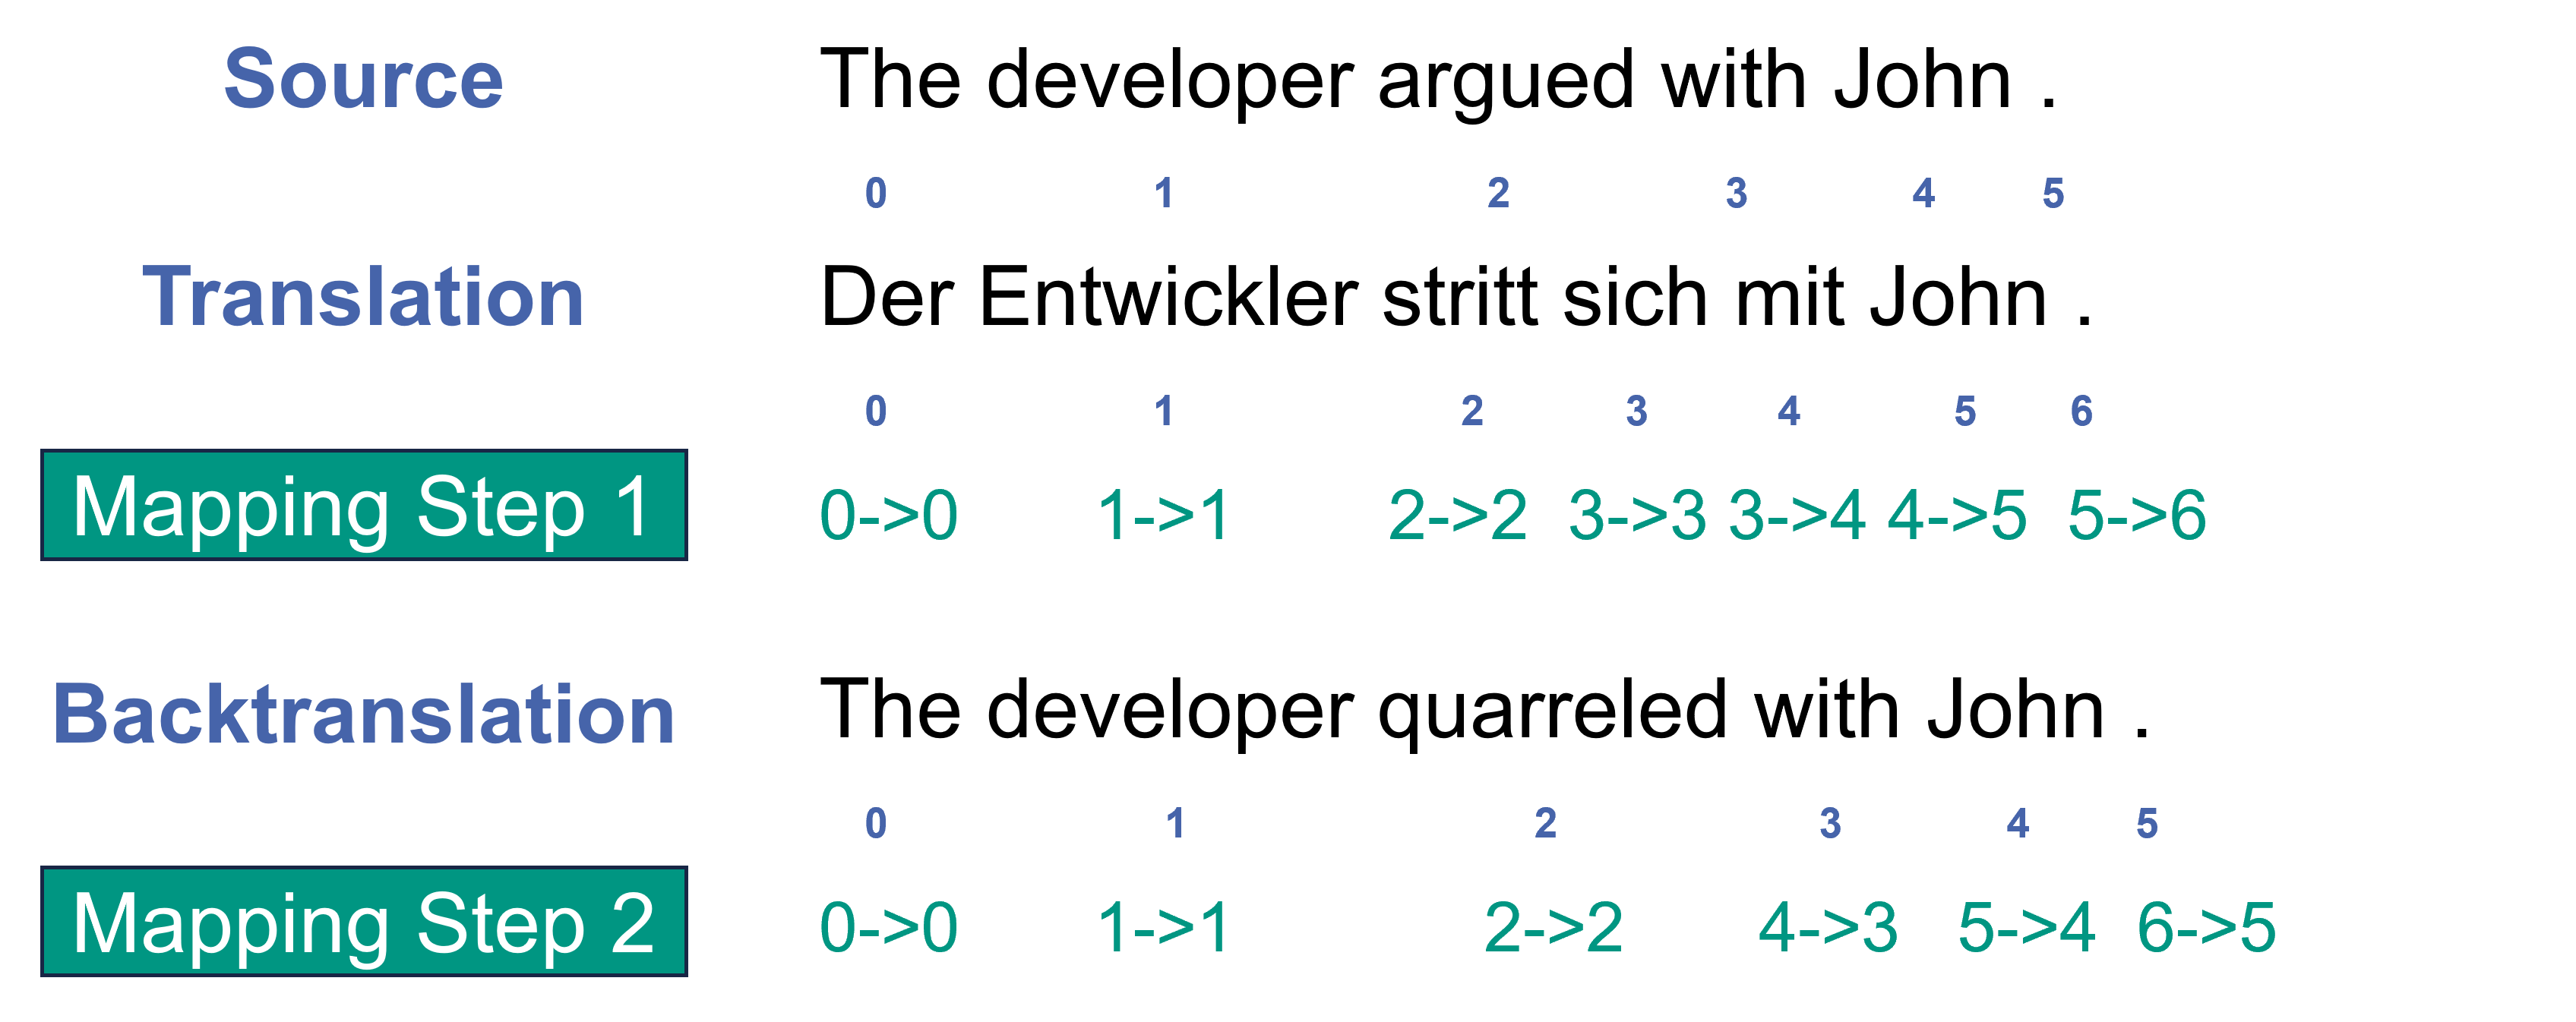
\includegraphics[scale=0.5]{figures/alignment.png}
  \caption{Example Illustration: 2-step mapping from source to translation and backtranslation}
  \label{fig:alignment}
\end{figure}

%%%%%%%%%%%%%%%%%%%%%%%%%%%%%%%%%%%%%%%%%%%%%%%%%
\subsection{Statistics}
\label{sec:Experiments:Statistics}

% TODO: define formally, maybe as a formula, pseudocode ???

We evaluate the translations and backtranslations of the subsets using a couple of statistical methods. We apply all methods to all subsets and compare the results of the subsets against each other.

%%%%%%%%%%%%%%%%%%%%%%%%
\subsubsection{Recurrence Evaluation}
\label{sec:Experiments:Statistics:Recurrence}
We evaluate how many of the source sentences and source words reoccur in the backtranslations:

\begin{enumerate}
    \item[1. ] Gather the backtranslations for each source sentences.
    \item[2a. ] Count the number of source sentences that reappear in their list of backtranslations
    \item[2b. ] Count the number of source sentences which contain the source word in their list of backtranslations
\end{enumerate}

The purpose of this evaluation is to determine which of the subsets are able to reconstruct more of the original source sentences/words.

%%%%%%%%%%%%%%%%%%%%%%%%
\subsubsection{Uniqueness Evaluation}
\label{sec:Experiments:Statistics:Uniqueness}
We evaluate the number of unique words and sentences in the translations and backtranslations for each sentence of the subsets. 

For the sake of the evaluation, we follow this routine (\textit{[translations | backtranslations]} denotes that we follow the same step for both the translations and backtranslations):
\begin{enumerate}
    \item[1. ] Collect the \textit{[translations | backtranslations]} for each source sentences.
    % sentence level
    \item[2a. ] Count how many of the \textit{[translations | backtranslations]} are unique. 
    % word level
    \item[2b. ] Count how many unique words there are in the \textit{[translations | backtranslations]} and normalize the number by the total amount of words. 
    \item[3. ] Average the result for all sentences.
\end{enumerate}

We use this method to probe the Hypotheses \ref{a} and \ref{b}. 

%%%%%%%%%%%%%%%%%%%%%%%%
\subsubsection{Alignment Evaluation}
\label{sec:Experiments:Statistics:Alignment}
Another form of evaluation is based on the alignment of the words between the source sentence, the translations and backtranslations (see Subsection \ref{sec:Experiments:Alignment} for more detail).

First, we align each word in the source sentence with its corresponding word in the translations and backtranslations. Then, to assess the translations and backtranslations of the source word, we do:
\begin{enumerate}
    \item[1. ] Collect all \textit{[translations | backtranslations]} of the source word.
    \item[2. ] Count how many of the \textit{[translations | backtranslations]} are unique.
    \item[3. ] Average the result for all sentences.
\end{enumerate}

Similarly, to assess the translations and backtranslations of the rest of the sentence excluding the source word, we do:
\begin{enumerate}
    \item[1. ] Collect all \textit{[translations | backtranslations]} of the sentence rest.
    \item[2. ] Count how many of the \textit{[translations | backtranslations]} are unique.
    \item[3. ] Average the result for all sentences.
\end{enumerate}

The idea behind this evaluation method is to assess the Hypothesis \ref{c}.

%%%%%%%%%%%%%%%%%%%%%%%%
\subsubsection{Gender Evaluation}
\label{sec:Experiments:Statistics:Gender}
We perform the evaluation of gender on the translations of the subsets.  For this purpose, the following steps are executed:

\begin{enumerate}
    \item[1. ] Gather the translations of the source word for each source sentence.
    \item[2. ] Detect the gender of the translations for each source sentence.
    \item[3a. ] Count how many of the source sentences produce \textit{both genders}, how many - \textit{female} and how many - \textit{male}. 
    \item[3b. ] Calculate how many of the translations are female and how many - male and determine the percent of the source sentences producing \textit{male} versus \textit{female}. 
\end{enumerate}

The purpose of this method is to assess if the translations produce the right gender (in disambiguated subsets) or both genders (in the original ambiguous subset).

In the next chapter, we will present the results of these statistical evaluations of the subsets.


